\documentclass{article}

\usepackage[dutch]{babel}
\usepackage[margin=3cm]{geometry}
\usepackage{graphicx}
\usepackage{float}
\usepackage{caption}
\usepackage{hyperref}
\usepackage{amsmath}
\usepackage{wrapfig}
\usepackage[parfill]{parskip}
\usepackage{eso-pic}

% fonts
\usepackage[T1]{fontenc}
\usepackage{helvet}
\renewcommand{\familydefault}{\sfdefault}

\graphicspath{{img/}}


% code
\usepackage{minted}
\setminted{frame=single,framesep=3pt,linenos}
\usepackage{upquote}
\usepackage{color}

\definecolor{titlepagecolor}{RGB}{68,200,245}

\begin{document}

\begin{titlepage}
    \pagecolor{titlepagecolor}
    \newgeometry{left=3cm,right=1cm,bottom=1cm}
    \noindent
\begin{flushright}
\vspace*{5cm}
 \vspace{2cm}
\end{flushright}
    \color{white}
    \par
    \noindent
    \color{white}
    \makebox[0pt][l]{\rule{1.3\textwidth}{1pt}}
    \par\medskip
    {\noindent \Huge\textbf{\textsf{User guide: Research project}}}
    \par\medskip
    {\noindent\Large\textsf{Pieter Specenier}}
    \par  
\vfill%


\end{titlepage}
\restoregeometry

\nopagecolor 

\pagenumbering{gobble}
\tableofcontents
\newpage

\pagenumbering{arabic}

% Add watermark to background of every page
\AddToShipoutPicture{
    \ifnum\value{page}>0
    \AtPageLowerLeft{
    \raisebox{3\baselineskip}{\makebox[0.25\paperwidth]{
        \begin{minipage}{21cm}\centering
            
\includegraphics{img/background.png}
        \end{minipage}}}
    }
  \fi
}

\section{Usage of API}
This document will tell you how to use the API. 
If you haven't yet gone through the installation guide please do so first.
\begin{enumerate}
    \item After installing everything you should now have access to this website.
    \begin{figure}[H]
        \centering
        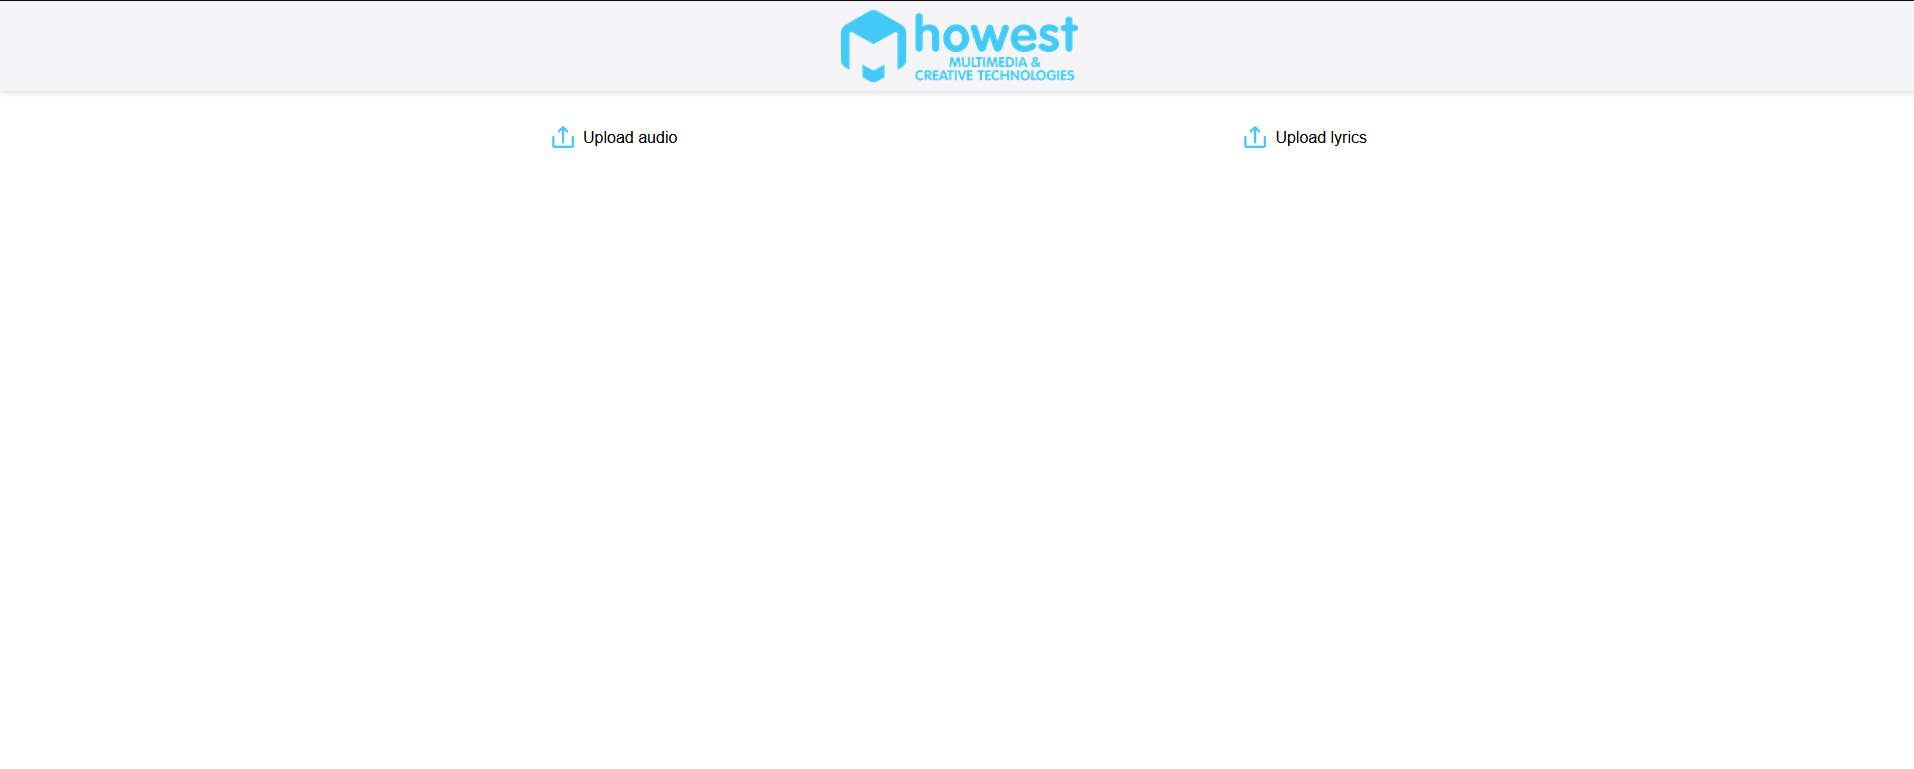
\includegraphics[width=0.6\textwidth]{website.PNG}
        \caption{View of the website}
    \end{figure}
    \item You can now either choose to click on the Upload lyrics button or on the Upload audio button.
    \item For lyrics you will have to enter an amount of words that you choose yourself the more the better the model can predict the genre of the lyrics!
    \begin{figure}[H]
        \centering
        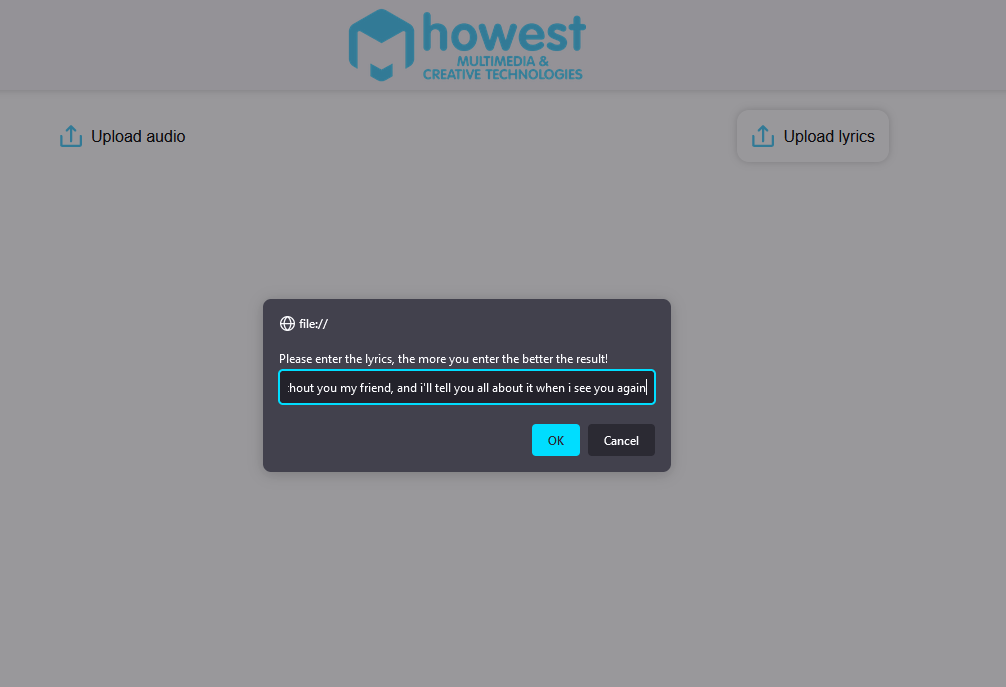
\includegraphics[width=0.6\textwidth]{lyricsmodel.PNG}
        \caption{Uploading lyrics}
    \end{figure}
    \item For audio you will have to upload an audio file please note that only .wav files are supported at the moment!
    \begin{figure}[H]
        \centering
        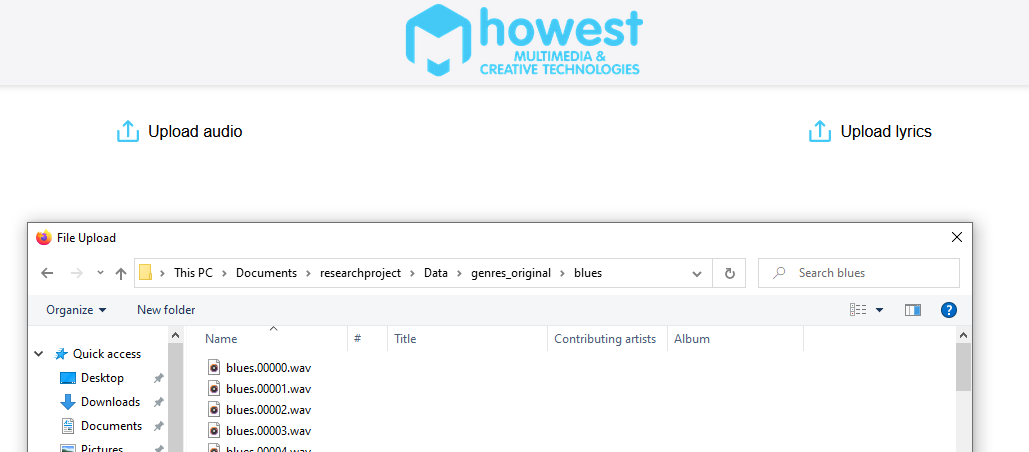
\includegraphics[width=0.6\textwidth]{audiomodel.PNG}
        \caption{Uploading an audio file}
    \end{figure}
    \item After doing either of the above you will be shown the results of the prediction along with three songs that are in the same genre of the audio or lyrics that you uploaded.
    \begin{figure}[H]
        \centering
        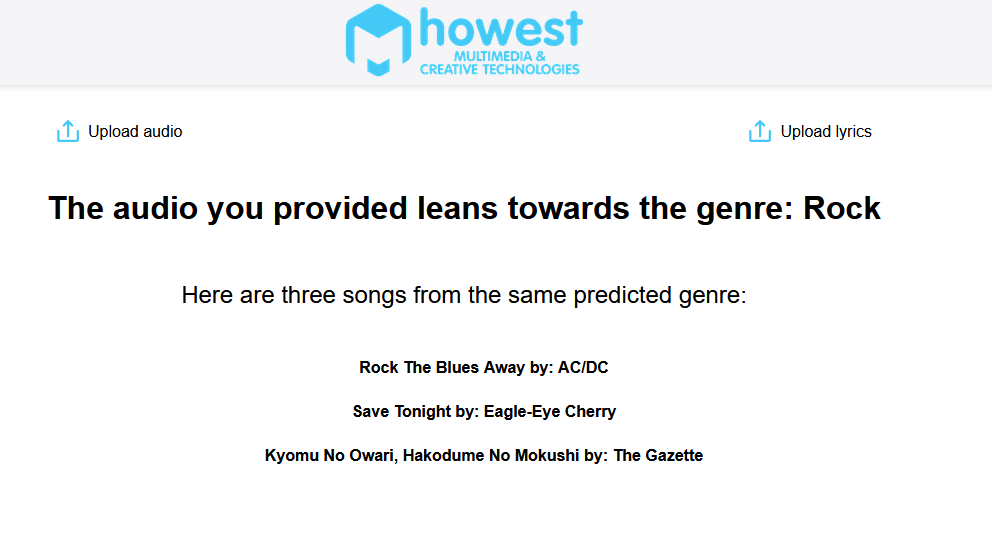
\includegraphics[width=0.7\textwidth]{audioprediction.PNG}
        \caption{Results of the model prediction}
    \end{figure}
\end{enumerate}


\end{document}